\documentclass[../main.tex]{subfiles}
\graphicspath{{\subfix{../diagrams/}}}


\begin{document}

\section{AlexCore}
Add text here

\subsection{Core Architecture}
Add text here

\subsection{Arithmetic Pipelines}
Add text here

\subsection{Handling Hazards}
Add text here

\subsection{Privilege ISA and CSRS}
RISC-V provides privilege architecture which includes privileged instructions as well as additional functionality required for running operating system and attaching external device.

\subsubsection*{RISC-V Privileged Software Stack Terminology}
\\The RISC-V ISA defines a wide range of possible privileged software stacks.
\begin{figure}[h]
\centering
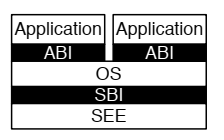
\includegraphics[width=5cm]{diagrams/risc_v_stack.png}
\caption{conventional operating system}
\label{fig:software_stack}
\end{figure}
Since we targeted to run OS on our RISC-V core we intended to use the following configuration as shown in figure
\ref{fig:software_stack} that can support multi-programmed execution of multiple applications. Each application communicates over an application binary interface (ABI) with the OS. RISC-V
operating systems interface with a supervisor execution environment (SEE), This environment consists of the supervisor-mode instructions and CSRs defined by the privileged ISA document.

\subsubsection*{Privilege Levels}
As described in the privileged ISA document, a RISC-V hardware thread (hart) is running at some privilege level encoded as a mode in one or more CSRs (control and status registers). there are three privilege levels are defined as shown in table \ref{tab:modes}. These privilege levels are used to provide protection between different components of the software stack, and attempts to perform operations not permitted by the current privilege mode will cause an exception to be raised. These exceptions will normally cause traps into an underlying execution environment.\\
\\The machine level has the highest privileges and is the only mandatory privilege level for a RISC-V hardware platform, As this is the only mode that has unfettered access to the whole machine. But since we need to run OS we implemented the other two modes (S, U).

\begin{table}[h]
\begin{center}
\begin{tabular}{ |c|c|c|c| } 
\hline
Level & Encoding & Name & Abbreviation \\
\hline
\multirow 
0 & 00 & User/Application & U \\ 
1 & 01 & Supervisor & S \\ 
2 & 10 & Reserved &  \\ 
3 & 11 & Machine & M \\
\hline
\end{tabular}
\end{center}
\caption{RISC-V privilege levels.}
\label{tab:modes}
\end{table}

\subsubsection*{Control and Status Registers (CSRs)}
Control and status register (CSR) is a register that stores various information in CPU. RISC-V defines a separate address space of 4096 CSRs so we can have at most 4096 CSRs. RISC-V only allocates a part of address space so we can add custom CSRs in unused addresses. Also, not all CSRs are required on all implementations.\\By convention, the upper 4 bits of the CSR address (csr[11:8]) are used to encode the read and write accessibility of the CSRs according to privilege level as shown in Table 2.1. The top two bits (csr[11:10]) indicate whether the register is read/write (00, 01, or 10) or read-only (11). The next two bits (csr[9:8]) encode the lowest privilege level that can access the CSR.\\ In our micro-architecture we only implement the required CSRs for the the modes to support interrupt handler and exceptions in addition to the timer interrupts registers. Also we implemented four custom CSRs for the crypto-IP integration.
The implemented CSR registers are listed in tables \ref{tab:CSRs} and \ref{tab:CSRs2} with there addresses and their names in our code.

\begin{table}[h!]
\centering

\begin{tabular}{|c|c|c|c|} 
\hline
CSR address & Privilege & Name & Description \\
\hline
\multicolumn{4}{|c|}{User Trap Setup}\\
\hline
0x000 & URW & CSR\_USTATUS & User status register\\
0x004 & URW & CSR\_UIE & User interrupt-enable register\\
0x005 & URW & CSR\_UTVEC & User trap-handler base address\\
\hline
\multicolumn{4}{|c|}{User Trap Handling}\\
\hline
0x140 & URW & CSR\_USCRATCH & Scratch register for Supervisor trap handlers\\
0x041 & URW & CSR\_UEPC & Supervisor exception program counter\\
0x042 & URW & CSR\_UCAUSE & Supervisor trap cause\\
0x043 & URW & CSR\_UTVAL & Supervisor bad address or instruction\\
0x044 & URW & CSR\_UIP & Supervisor interrupt pending\\
\hline
\multicolumn{4}{|c|}{User Counter/Timers}\\
\hline
0xC00 & URW & CSR\_CYCLE & Cycle counter for RDCYCLE instruction\\
0xC01 & URW & CSR\_TIME & Timer for RDTIME instruction\\
0xC02 & URW & CSR\_INSTERT & counter for RDINSTRET instruction\\
0x8FF & URW & CSR\_UNECYCLE & User timer\\
\hline
\multicolumn{4}{|c|}{Supervisor Trap Setup}\\
\hline
0x100 & SRW & CSR\_SSTATUS & Supervisor status register\\
0x102 & SRW & CSR\_SEDELEG & Supervisor exception delegation register\\
0x103 & SRW & CSR\_SIDELEG & Supervisor interrupt delegation register\\
0x104 & SRW & CSR\_SIE & Supervisor interrupt-enable register\\
0x105 & SRW & CSR\_STVEC & Supervisor trap-handler base address\\
0x106 & SRW & CSR\_SCOUNTEREN & Supervisor counter enable\\
\hline
\multicolumn{4}{|c|}{Supervisor Trap Handling}\\
\hline
0x140 & SRW & CSR\_SSCRATCH & Scratch register for Supervisor trap handlers\\
0x141 & SRW & CSR\_SEPC & Supervisor exception program counter\\
0x142 & SRW & CSR\_SCAUSE & Supervisor trap cause\\
0x143 & SRW & CSR\_STVAL & Supervisor bad address or instruction\\
0x144 & SRW & CSR\_SIP & Supervisor interrupt pending\\
\hline
\multicolumn{4}{|c|}{Machine Information Registers}\\
\hline
0xF11 & MRO & CSR\_MVENDORID & Vendor ID \\ 
0xF12 & MRO & CSR\_MARCHID & Architecture ID \\ 
0xF13 & MRO & CSR\_MIMPID &  Implementation ID\\ 
0xF14 & MRO & CSR\_MHARTID & Hardware thread ID\\
\hline
\multicolumn{4}{|c|}{Machine Trap Setup}\\
\hline
0x300 & MRW & CSR\_MSTATUS & Machine status register\\
0x301 & MRW & CSR\_MISA & ISA and extensions\\
0x302 & MRW & CSR\_MEDELEG & Machine exception delegation register\\
0x303 & MRW & CSR\_MIDELEG & Machine interrupt delegation register\\
0x304 & MRW & CSR\_MIE & Machine interrupt-enable register\\
0x305 & MRW & CSR\_MTVEC & Machine trap-handler base address\\
0x306 & MRW & CSR\_MCOUNTEREN & Machine counter enable\\
\hline
\multicolumn{4}{|c|}{Machine Trap Handling}\\
\hline
0x340 & MRW & CSR\_MSCRATCH & Scratch register for machine trap handlers\\
0x341 & MRW & CSR\_MEPC & Machine exception program counter\\
0x342 & MRW & CSR\_MCAUSE & Machine trap cause\\
0x343 & MRW & CSR\_MTVAL & Machine bad address or instruction\\
0x344 & MRW & CSR\_MIP & Machine interrupt pending\\
\hline
\end{tabular}
\caption{Implemented CSRs.}
\label{tab:CSRs}
\end{table}

\begin{table}[t!]
\centering
\begin{tabular}{ |c|c|c|c| } 
\hline
CSR address & Privilege & Name & Description \\
\hline
\multicolumn{4}{|c|}{Machine Counter/Timers}\\
\hline
0xB00 & MRW & CSR\_MCYCLE & Machine cycle counter\\
0xB02 & MRW & CSR\_MINSTRET & Machine instructions-retired counter\\
0xB80 & MRW & CSR\_MCYCLEH & Upper 32 bits of mcycle, RV32I only\\
0xB82 & MRW & CSR\_MCYCLEH & Upper 32 bits of minstret, RV32I only\\
\hline
\multicolumn{4}{|c|}{Custom CSRs for the Encryption IP}\\
\hline
0x7C0 & MRW & CSR\_AES\_D0 & lowest 32 bits of data\\
0x7C1 & MRW & CSR\_AES\_D1 & data from 32:63\\
0x7C2 & MRW & CSR\_AES\_D2 & data from 64:95\\
0x7C3 & MRW & CSR\_AES\_D3 & highest 32 bits of data\\
0x7C4 & MRW & CSR\_AES\_key & key address\\
\hline
\end{tabular}
\caption{Implemented CSRs.}
\label{tab:CSRs2}
\end{table}

\subsubsection*{“Zicsr”, Control and Status Register Instructions}
This extension defines the full set of CSR instructions that operate on the CSRs.\\
\\All CSR instructions atomically read-modify-write a single CSR, whose CSR specifier is encoded in the 12-bit csr field of the instruction held in bits 31–20. The immediate forms use a 5-bit zero-extended immediate encoded in the rs1 field as shown in fig \ref{fig:csr_inst}.
\begin{figure}[t]
\centering
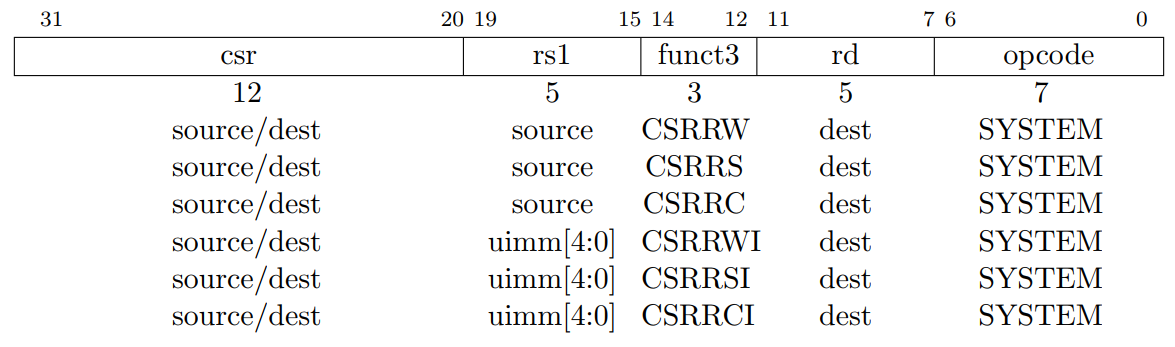
\includegraphics[width=15 cm]{diagrams/csr_inst.png}
\caption{CSR Instructions}
\label{fig:csr_inst}
\end{figure}
The CSRRW (Atomic Read/Write CSR) instruction atomically swaps values in the CSRs and integer registers. CSRRW reads the old value of the CSR, zero-extends the value to XLEN bits, then writes it to integer register rd. The initial value in rs1 is written to the CSR. If rd=x0, then the instruction shall not read the CSR and shall not cause any of the side effects that might occur
on a CSR read.\\
\\The CSRRS (Atomic Read and Set Bits in CSR) instruction reads the value of the CSR, zeroextends the value to XLEN bits, and writes it to integer register rd. The initial value in integer register rs1 is treated as a bit mask that specifies bit positions to be set in the CSR. Any bit that is high in rs1 will cause the corresponding bit to be set in the CSR, if that CSR bit is writable. Other bits in the CSR are unaffected (though CSRs might have side effects when written).\\
\\The CSRRC (Atomic Read and Clear Bits in CSR) instruction reads the value of the CSR, zeroextends the value to XLEN bits, and writes it to integer register rd. The initial value in integer register rs1 is treated as a bit mask that specifies bit positions to be cleared in the CSR. Any bit that is high in rs1 will cause the corresponding bit to be cleared in the CSR, if that CSR bit is writable. Other bits in the CSR are unaffected.\\
\\For both CSRRS and CSRRC, if rs1=x0, then the instruction will not write to the CSR at all, and so shall not cause any of the side effects that might otherwise occur on a CSR write, such as raising
illegal instruction exceptions on accesses to read-only CSRs. Both CSRRS and CSRRC always read the addressed CSR and cause any read side effects regardless of rs1 and rd fields. Note that if rs1
specifies a register holding a zero value other than x0, the instruction will still attempt to write the unmodified value back to the CSR and will cause any attendant side effects. A CSRRW with
rs1=x0 will attempt to write zero to the destination CSR.\\
\\The CSRRWI, CSRRSI, and CSRRCI variants are similar to CSRRW, CSRRS, and CSRRC respectively, except they update the CSR using an XLEN-bit value obtained by zero-extending a 5-bit unsigned immediate (uimm[4:0]) field encoded in the rs1 field instead of a value from an integer register. For CSRRSI and CSRRCI, if the uimm[4:0] field is zero, then these instructions will not write to the CSR, and shall not cause any of the side effects that might otherwise occur on a CSR write. For CSRRWI, if rd=x0, then the instruction shall not read the CSR and shall not cause any of the side effects that might occur on a CSR read. Both CSRRSI and CSRRCI will always read the CSR and cause any read side effects regardless of rd and rs1 fields.

\subsubsection*{Machine-Level ISA}
This section describes the machine-level operations available in machine-mode (M-mode), which is the highest privilege mode in a RISC-V system, M-mode code can access all CSRs
at lower privilege levels. M-mode is used for low-level access to a hardware platform and is the first mode entered at reset.\\

\begin{itemize}
    \item[1- ]Machine-Level CSRs
        \begin{itemize}
            \item Machine ISA Register misa\\
            The misa CSR is a WARL read-write register reporting the ISA and extensions supported by the hart and implemented as shown in fig. \ref{fig:misa}.
            \begin{figure}[h]
            \centering
            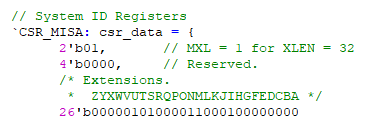
\includegraphics[width=10 cm]{diagrams/misa.png}
            \caption{misa register}
            \label{fig:misa}
            \end{figure}
            \item Machine Vendor ID Register mvendorid, Machine Architecture ID Register marchid, Machine Implementation ID Register mimpid & Hart ID Register mhartid\\
            These registers are hardwired to zero.\\
            \item Machine Status Register (mstatus)\\
            The mstatus register keeps track of and controls the hart’s current operating state.
            The main fields in the mstatus registers are shown in fig. \ref{fig:mstatus}
            \begin{figure}[h]
            \centering
            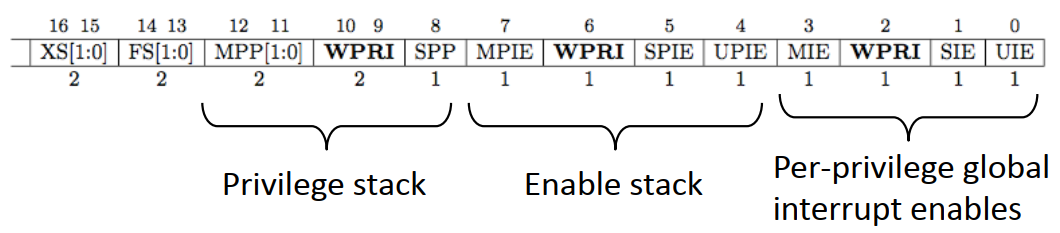
\includegraphics[width=10 cm]{diagrams/mstatus.png}
            \caption{mstatus register}
            \label{fig:mstatus}
            \end{figure}
            Global interrupt-enable bits, MIE, SIE, and UIE, are provided for each privilege mode. When a hart is executing in privilege mode x, interrupts are globally enabled when x IE=1 and globally disabled when x IE=0.\\
            Only take a pending interrupt for privilege mode x if xIE=1 and running in mode x or greater.
            The TSR (Trap SRET) bit supports intercepting the supervisor exception return instruction, SRET. When TSR=1, attempts to execute SRET while executing in S-mode will raise an illegal instruction exception. When TSR=0, this operation is permitted in S-mode.\\
            \begin{figure}[h]
            \centering
            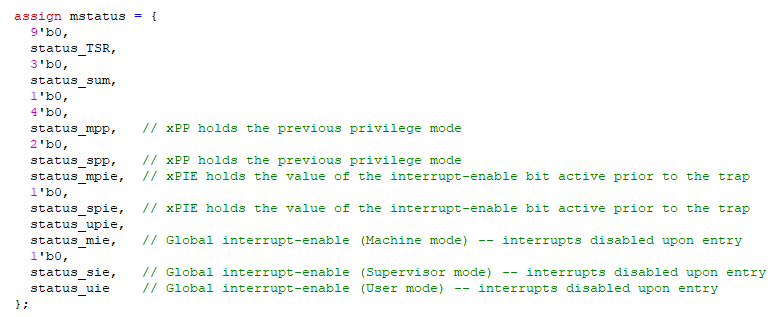
\includegraphics[width=15 cm]{diagrams/mstatus-imp.png}
            \caption{mstatus register implementation}
            \label{fig:mstatus-imp}
            \end{figure}
            Fig. \ref{fig:mstatus-imp} describes the implementation of the mstatus register in our core, the hardwired bits with zero indicates that these functions are not implemented.\\
            \item Machine Trap-Vector Base-Address Register (mtvec)\\
            The mtvec register is an MXLEN-bit read/write register that holds trap vector configuration, consisting of a vector base address (BASE) and a vector mode (MODE).
            There are two modes (Direct - Vectored)\\
            When MODE=Direct, all traps into machine mode cause the pc to be set to the address in the BASE field. When MODE=Vectored, all synchronous exceptions into machine mode cause the pc to be set to the address in the BASE field, whereas interrupts cause the pc to be set to the address in the BASE field plus four times the interrupt cause number and we will discuss cause number in mcause register.\\
            In our core we implemented the direct mode.\\
            \item Machine Trap Delegation Registers (medeleg and mideleg)\\
            
            \item Machine Interrupt Registers (mip and mie)\\
            
            \item Machine Scratch Register (mscratch)\\
            The mscratch is an MXLEN-bit read/write register\\
            Typically, it is used to hold a pointer to a machine-mode hart-local context space and swapped with a user register upon entry to an M-mode trap handler.\\
            
            \item Machine Exception Program Counter (mepc)\\
            When a trap is taken into M-mode, mepc is written with the address of the instruction that was interrupted or that encountered the exception. Otherwise, mepc is never written by the implementation, though it may be explicitly written by software.\\
            since our implementation supports only IALIGN=32, the two low bits (mepc[1:0]) are always zero.\\
            
            \item Machine Cause Register (mcause)\\
            When a trap is taken into M-mode, mcause is written with a code indicating the event that caused the trap. Otherwise, mcause is never written by the implementation, though it may be explicitly written by software.\\
            \begin{figure}[h]
            \centering
            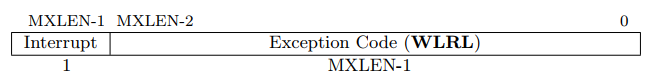
\includegraphics[width=10 cm]{diagrams/mcause.png}
            \caption{mcause register}
            \label{fig:mcause}
            \end{figure}As shown in fig. \ref{fig:mcause}
            The Interrupt bit in the mcause register is set if the trap was caused by an interrupt. The Exception Code field contains a code identifying the last exception. 
            fig. \ref{fig:exception-code} lists the possible machine-level exception codes.\\
            \begin{figure}[h!]
            \centering
            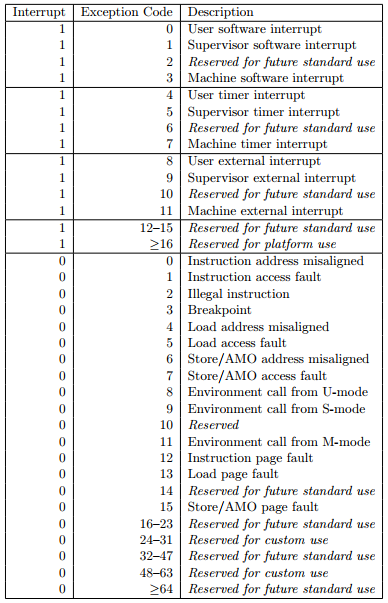
\includegraphics[width=10 cm]{diagrams/exception_code.png}
            \caption{exception codes}
            \label{fig:exception-code}
            \end{figure}
            
            \item Machine Trap Value (mtval) Register\\
            When a trap is taken into M-mode, mtval is either set to zero or written with exception-specific information to assist software in handling the trap. Otherwise, mtval is never written by the implementation, though it may be explicitly written by software. The hardware platform will specify which exceptions must set mtval informatively and which may unconditionally set it to zero.
        \end{itemize}
        
    \item[2- ]Machine-Mode Privileged Instructions
        \begin{itemize}
            \item Environment Call\\
            The ECALL instruction shown in fig. \ref{fig:ecall} is used to make a request to the supporting execution environment. When executed in U-mode, S-mode, or M-mode, it generates an environment-call-from-U-mode exception, environment-call-from-S-mode exception, or environment-call-from-M-mode exception, respectively, and performs no other operation.\\
            \begin{figure}[h!]
            \centering
            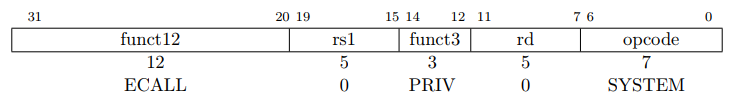
\includegraphics[width=10 cm]{diagrams/ecall.png}
            \caption{ECALL Instruction}
            \label{fig:ecall}
            \end{figure}
            
            \item Trap-Return Instructions\\
            To return after handling a trap, there are separate trap return instructions per privilege level: MRET, SRET, and URET shown in fig. \ref{fig:ret}.\\
            \begin{figure}[h!]
            \centering
            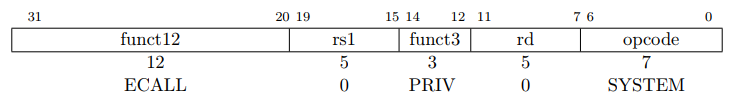
\includegraphics[width=10 cm]{diagrams/ecall.png}
            \caption{Return Instructions}
            \label{fig:ret}
            \end{figure}An xRET instruction can be executed in privilege mode x or higher, where executing a lower-privilege xRET instruction will pop the relevant lower-privilege interrupt enable and privilege mode stack. In addition to manipulating the privilege stack, xRET sets the pc to the value stored in the xepc register.
        \end{itemize}
    \item[3- ]Reset\\
    Upon reset, a hart’s privilege mode is set to M. The mstatus fields MIE and MPRV are reset to 0.
\end{itemize}

\subsection{Interrupt Controller}
RISC-V defines the following interrupts per Hart:
\begin{itemize}
    \item Software – architecturally defined software interrupt
    \item Timer – architecturally defined timer interrupt
    \item External – Peripheral Interrupts
\end{itemize}
\textbf{Core Local Interrupter (CLINT)}\\
The CLINT has a fixed priority scheme which implements Software, Timer, and External interrupts. Software preemption is only available between privilege levels using the CLINT. For example, while in Supervisor mode, a Machine mode interrupt will immediately take priority and preempt Supervisor mode operation. Preemption within a privilege level is not supported with the CLINT. The interrupt ID represents the fixed priority value of each interrupt, and is not configurable. There are two different CLINT modes of operation, direct mode and vectored mode. To configure CLINT modes, write mtvec.mode field, which is bit[0] of mtvec CSR. For direct mode, mtvec.mode=0, and for vectored mode mtvec.mode=1. Direct mode is the default reset value. The mtvec.base holds the base address for interrupts and exceptions, and must be a minimum 4-byte aligned value in direct mode.\\
In our design we used the direct mode, Direct mode means all interrupts and exceptions trap to the same handler, and there is no vector table implemented. It is software’s responsibility to execute code to figure out which interrupt occurred. The software handler in direct mode should first read mcause.interrupt to determine if an interrupt or exception occurred, then decide what to do based on mcause.code value which contains the respective interrupt or exception code.\\
\\The trap handler - entry and exit are performed as the following:
\begin{itemize}
    \item[1-]Save pc to mepc
    \item[2-]Save Privilege level to mstatus.mpp
    \item[3-]Save mie to mstatus.mpie
    \item[4-]Set pc to interrupt handler address, based on mode of operation
    \item[5-]Disable interrupts by setting mstatus.mie=0\\
    At this point control is handed over to software where the interrupt processing begins. At the end of the interrupt handler, the mret instruction will do the following.
    \item[6-]Restore mepc to pc
    \item[7-]Restore mstatus.mpp to Priv
    \item[8-]Restore mstatus.mpie to mie
\end{itemize}
\textbf{where priv refers to the current privilege level}

\end{document}